\documentclass[a4paper,10pt]{report}
\usepackage{geometry}\geometry{a4paper,top=3.5cm,bottom=3.5cm,%
left=2.5cm,right=2.5cm,heightrounded,bindingoffset=0mm}
\usepackage[T1]{fontenc}
\usepackage[utf8]{inputenc}
\usepackage[italian]{babel}
\usepackage{graphicx}
\usepackage[export]{adjustbox}%Per il Frame attrono le immagini e il valign
\usepackage{subfig}
\usepackage{amsmath,amsfonts,amssymb,braket,mathrsfs}
\usepackage{float}
\usepackage{tabularx,booktabs}
\usepackage{hyperref}
\usepackage{epsfig}
\usepackage{pdfpages} %Per gli allegati
%\usepackage{minipage}
\usepackage[output-decimal-marker={,}]{siunitx}
\usepackage{tikz}
\usepackage{pgfplots,pgfplotstable}
%\pgfplotsset{compat=1.15} %indica la versione da utilizzare per pgfplot
\usetikzlibrary{patterns} % per il tratteggio
\usepgfplotslibrary{groupplots}
\pgfplotsset{compat=newest}
%\usepackage{stanli}
\usepackage{xspace}% per lo spazio intelligente
\newcommand{\e}{\`E\xspace}  %E'
\usepackage{titlesec} % per formato custom dei titoli dei capitoli
%\usepackage{sideways}%%%
% redefinizione del formato del titolo del capitolo
      % da formato
      %   Capitolo X
      %   Titolo capitolo
      %   a formato
      %      Titolo capitolo 
	\titleformat{\chapter}
        {\normalfont\Huge\bfseries}{}{0em}{}
	\titlespacing*{\chapter}{0pt}{0in}{0.02in}
	\titlespacing*{\section}{0pt}{0.2in}{0.02in}
	\titlespacing*{\subsection}{0pt}{0.10in}{0.02in}
%serve per la didascalia di tabelle e figure:
\usepackage{caption}
\captionsetup{tableposition=top,figureposition=bottom,font=small}\captionsetup{format=hang,labelfont={bf,color=pantone186}} %didascalie a più righe allineate e il nome in grassetto
%non viene allineato a sinistra se la didascalia è corta una sola riga. PERCHé??
\usepackage{xcolor}
%serve per mettere il codice con lo sfondo grigio chiaro
\definecolor{pantone186}{RGB}{206, 17, 38} %il colore del logo UNITN
\definecolor{myGray}{gray}{0.5} %più basso più scuro è
\usepackage{listings} 
\lstset{basicstyle=\scriptsize\ttfamily,
backgroundcolor=\color{lightgray},%
boxpos=c,%
stringstyle=\itshape,		
lineskip=3pt,%
numbers=left,
numberstyle=\tiny,}
\usepackage{lscape}
\usepackage{multirow}
\usepackage{import}
%\usepackage{pythontex}
\begin{document}
%!TEX root = ../TesiTriennaleMeoliNicola.tex
\pagestyle{plain}
\thispagestyle{empty}
\begin{center}
  \begin{figure}[H]
    \centerline{
\psfig{file=IMG/logo_unitn_black_centerNEW.eps,
                        width=0.8\textwidth,trim = 0 0.9cm 0 0.5cm}}
  \end{figure}
\textcolor{pantone186}{\noindent\rule{\textwidth}{.5pt}}

  \Large\textsc{Dipartimento di Ingegneria Civile, Ambientale e Meccanica\\}
  \Large{Corso di Laurea in Ingegneria Civile
  }

  \vspace{3.7 cm} 
  %\Large\textsc{Elaborato finale\\} 
  %\vspace{1 cm} 
  \Huge\textsc{Confronto energetico tra diverse soluzioni edilizie\\}
  
  \vspace{0.2 cm}
  \Large{\it{Analisi termo igrometrica di alcuni pacchetti strutturali composti da differenti materiali. }}


  \vspace{4 cm} 
  \begin{tabular*}{\textwidth}{ l @{\extracolsep{\fill}} r }
  \Large\textsc{Docenti} & \Large\textsc{Studente}\\
  \Large{Rossano Albatici}& \Large{Nicola Meoli 186100}\\
  
  	
  	
  \end{tabular*}

  \vspace{3.1cm} 
  \textcolor{pantone186}{\noindent\rule{\textwidth}{1pt}}
    
  \Large{Anno accademico 2020/21}
  
\end{center}


\tableofcontents
%\setcounter{page}{1}
%Tabelle e figure sulla stessa pagina:
%Le aggiunge all'indice. phantomsection serve per non far casini con hyperref
\clearpage
\begingroup
   %\let\cleardoublepage\relax  % book
    \let\clearpage\relax        % report
        \listoftables
        \phantomsection
        \addcontentsline{toc}{chapter}{Elenco delle tabelle}
        %
        \listoffigures
        \phantomsection
        \addcontentsline{toc}{chapter}{Elenco delle figure}
\endgroup
%

\chapter{nome capitlo 1}
\begin{figure}[htbp]
    \centering
    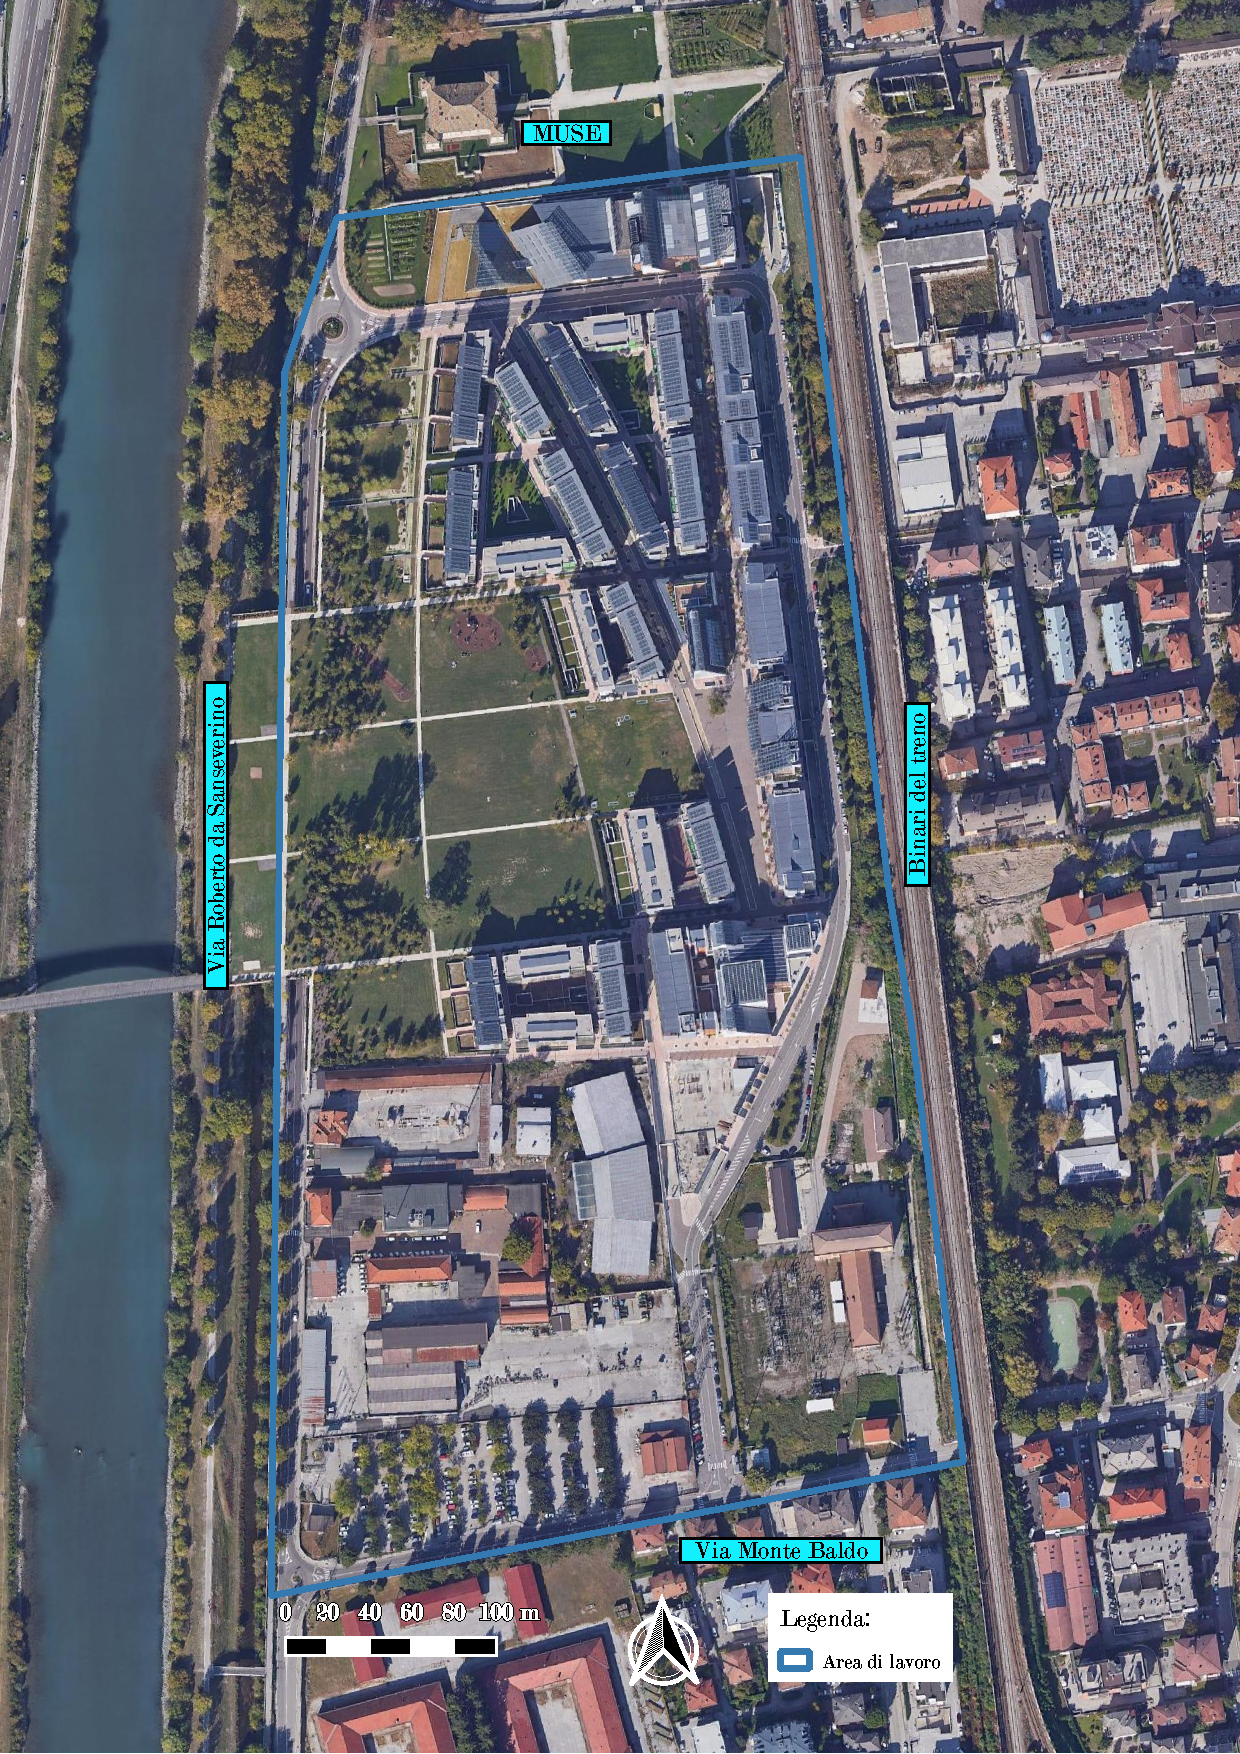
\includegraphics[trim=0cm 0cm 0cm 0cm,clip,frame,width=\textwidth]{IMG/inquadramento.pdf} 
    \caption{Inquadramento dell'area di lavoro}
    \label{fig:inquadramento}
    \end{figure}

\begin{equation}
    i = a \, t_p ^{n - 1}
\end{equation}
\begin{equation}
    CN = \frac{25400}{254 + S}
\end{equation}

\begin{equation}
    T_{\text{dry}} = \frac{3.125}{\sqrt{K_s}}
\end{equation}
Dove $T_{\text{dry}}$ sono i giorni che impiega il suolo completamente saturo a tornare secco e $K_s$ è la conduttività idraulica espressa in \si{inch\per\hour}.
\begin{equation}
    i_m = \frac{h(t_\text{fin}) - h(t_\text{in})}{\Delta t}
\end{equation}
\begin{equation}   
    h(t) = 
    \begin{cases}
        r \, a \left[ \left( \frac{t_p}{r}\right)^n - \left( \frac{t_p - t}{r}\right)^n  \right] & \text{se $t < t_p$}\\
        a \left[ r \left( \frac{t_p}{r}\right)^n + (1-r)\left( \frac{t_p - t}{1 - r}\right)^n  \right] & \text{se $t > t_p$}\\
    \end{cases}
\end{equation}
 


















\begin{landscape}
    \begin{figure}[htb]
        \centering
        \begin{tikzpicture}
            \begin{axis}[
                restrict x to domain=-0:1.5,
                height=15cm,
                width=21cm,
                grid=major,
                xlabel=Tempo trascorso dall'inizio della precipitazione \si{[\hour]},
                ylabel=Deflusso  \si{[\litre\per\second]},
                xtick = {0.5,1,1.5,2,2.5,3,3.5,4},
                %title= ,
                /pgf/number format/.cd,
                use comma,
                1000 sep={\,}
            ]
            \addplot +[mark=none,style=solid,color=red] table[x index=0,y index=1,header=false] {IMG/Total-Inflow/total_inflow_1min.txt};
            \addplot +[mark=none,style=solid,color=green!60!black] table[x index=0,y index=1,header=false] {IMG/Total-Inflow/total_inflow_2min.txt};
            \addplot +[mark=none,style=solid,color=magenta] table[x index=0,y index=1,header=false] {IMG/Total-Inflow/total_inflow_5min.txt};
            \addplot +[mark=none,style=solid,color=cyan] table[x index=0,y index=1,header=false] {IMG/Total-Inflow/total_inflow_10min.txt};
            \addplot +[mark=none,style=solid,color=orange] table[x index=0,y index=1,header=false] {IMG/Total-Inflow/total_inflow_15min.txt};
            \addplot +[mark=none,style=solid,color=teal] table[x index=0,y index=1,header=false] {IMG/Total-Inflow/total_inflow_30min.txt};
            \addplot +[mark=none,style=solid,color=violet] table[x index=0,y index=1,header=false] {IMG/Total-Inflow/total_inflow_45min.txt};
            \legend{1 min,2 min,5 min,10 min,15 min,30 min,45 min}    
            \end{axis}
        \end{tikzpicture}
        \caption{Deflusso del bacino}
        \label{fig:Ietogrammi}
    \end{figure}
\end{landscape}

\begin{landscape}
    \begin{figure}[htb]
        \centering
        \begin{tikzpicture}
            \begin{axis}[
                restrict x to domain=-0:4,
                height=15cm,
                width=21cm,
                grid=major,
                xlabel=Tempo trascorso dall'inizio della precipitazione \si{[\hour]},
                ylabel=Total Inflow  \si{[\litre\per\second]},
                xtick = {0.5,1,1.5,2,2.5,3,3.5,4},
                %title= ,
                /pgf/number format/.cd,
                use comma,
                1000 sep={\,}
            ]
            \addplot +[mark=none,style=solid,color=red] table[x index=0,y index=1,header=false] {IMG/Total-Inflow/total_inflow_5min_Chicago_25anni.txt};
            \end{axis}
        \end{tikzpicture}
        \caption{Andamento dello sforzo assiale agente sul pilastro P27 in funzione dell'altezza}
        \label{fig:IetogrammaFinale}
    \end{figure}   
\end{landscape}

\end{document}